% !TEX root = ../main.tex
\documentclass[../main.tex]{subfiles}
\begin{document}
\label{sec:results}

In this Section we explore the consistency with which volunteers modelled galaxies, the variance of the aggregate model recovered and how well our recovered models agree with other results in the literature.


\subsection{Examination of Volunteer consistency}
Figure \ref{fig:volunteer_component_consistency} illustrates the consistency with which volunteers made use of a component in their model for a galaxy. We see that volunteer classification is quite consistent, with volunteers almost always using a disk and bulge, and consistent proportions agreeing on the presence of a bar and the number of spiral arms.

\begin{figure*}
  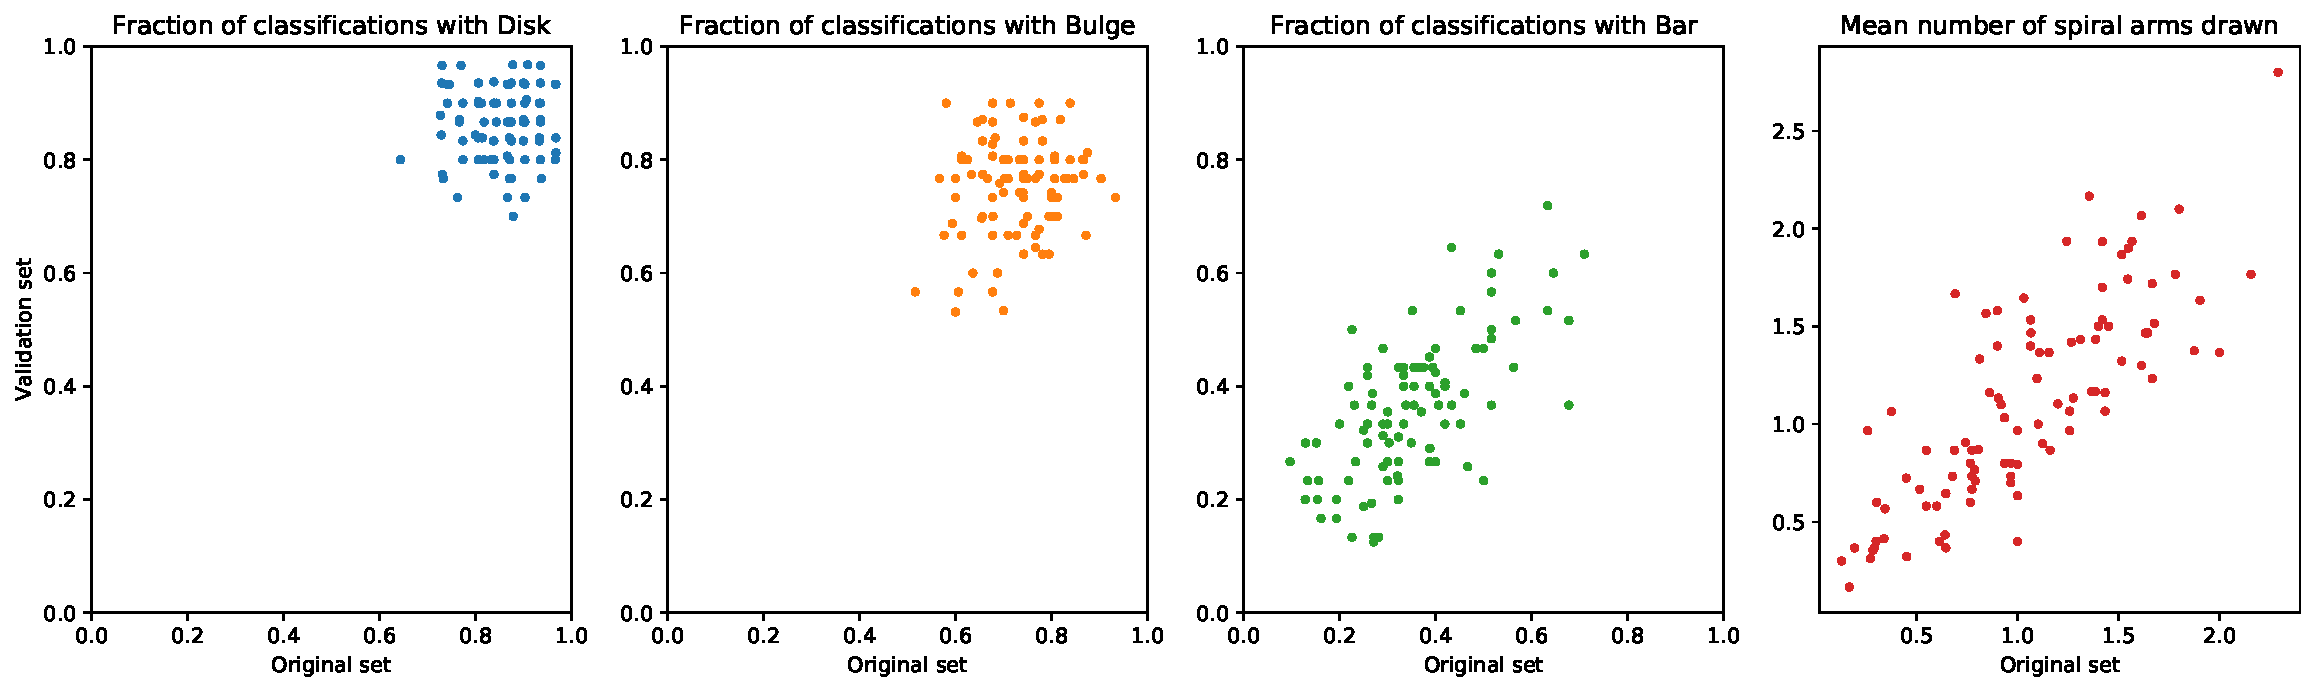
\includegraphics[width=17.3cm]{images__results/component_frequency.pdf}
  \caption{Comparison of frequency of use of component in volunteer models between the original and validation sets of classifications.}
  \label{fig:volunteer_component_consistency}
\end{figure*}

Regarding the components present in the aggregate models, we see some consistency in isophotal shape and size, as shown in Figure \ref{fig:aggregate_model_consistency}. The least consistent component is the bar. This may be due to the low proportion of volunteers incorporating one into their model (as illustrated in Figure. \ref{fig:volunteer_component_consistency}, visual inspection suggests that many volunteers used a very elliptical bulge and drawn spirals to capture the light from the bar). Fewer bars drawn by volunteers also has the effect of making clustering more difficult and more uncertain, even for a strongly barred galaxy we effectively go from receiving 30 classifications to around 12.

\begin{figure*}
  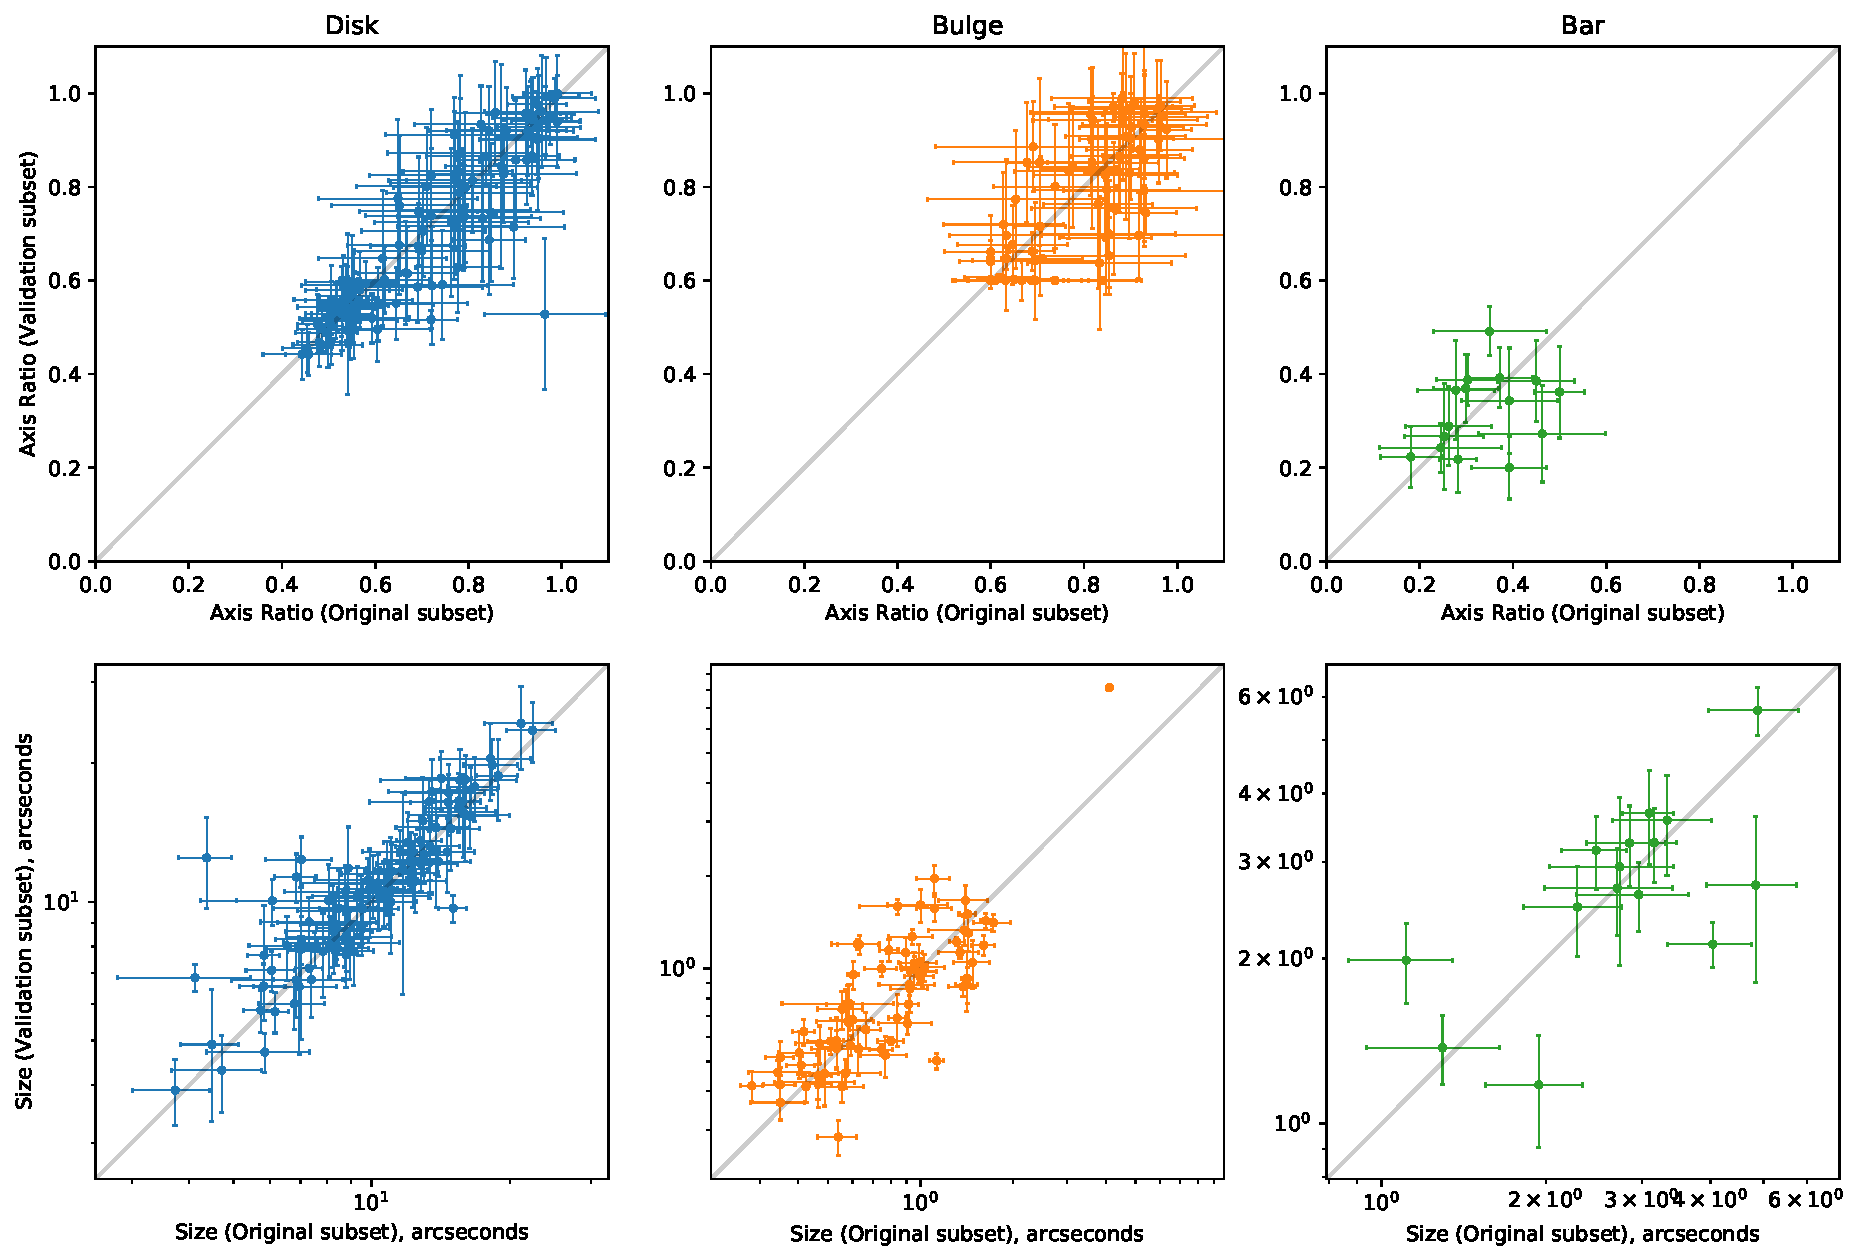
\includegraphics[width=17.3cm]{images__results/component_sizing.pdf}
  \caption{Comparison of component shape in aggregate models between the original and validation sets.}
  \label{fig:aggregate_model_consistency}
\end{figure*}

% We also combine classifications from the original and validation subsets and repeatedly draw 30 classifications from the pool to calculate an aggregate model and examine the variation in calculated models. Figure \ref{fig:aggregate_model_ss_variance} illustrates the consistency of components in models; we
% \begin{figure*}
%   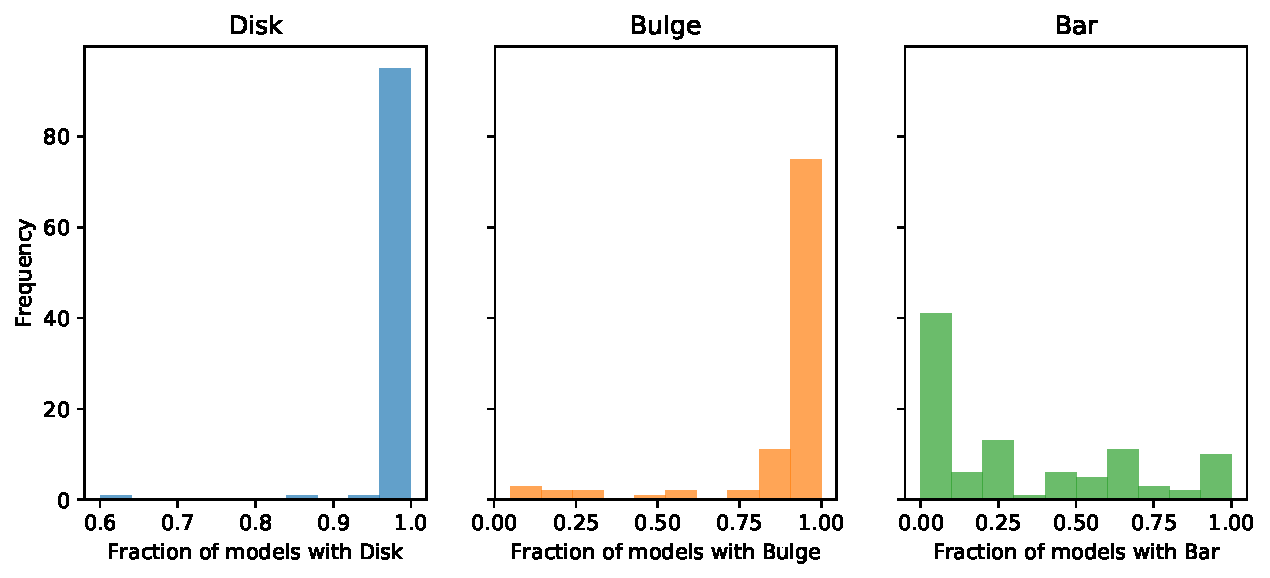
\includegraphics[width=17.3cm]{images__results/model-consistency-comparison.pdf}
%   \caption{Examination of how consistently components appear in aggregate models. Given a pool of 60 classifications for a galaxy, we repeatedly sample 30 classifications and calculate an aggregate model. We then obtain a fraction of these models containing each available component, which has been histogrammed. If our models were perfectly resilient (i.e. consistent components regardless of sampled classification), we would see two peaks at 0.0 and 1.0; the presence of galaxies with intermediate fractions suggests that the presence of a component in our model has some uncertainty.}
%   \label{fig:aggregate_model_ss_variance}
% \end{figure*}

\subsection{Comparison to results in the literature}
\subsubsection{Aggregated Disk, Bulge and Bar}
After having obtained aggregated models for our galaxies, we examine the reliability of our models through comparison to other results in the literature. For instance, if we compare the axis ratios of the disks recovered from Galaxy Builder to the axis ratio of a 2D S\'ersic fit to the r-band SDSS image of each galaxy (as provided in the NASA-Sloan Atlas), we see excellent agreement (Figure \ref{fig:ax_ratio_comparison}). We note that the results from Galaxy Builder tend to prefer a slightly more elliptical axis ratio, but plateau at an axis ratio of $0.5$. This could be due to the drawing tool ellipse having a default axis ratio of $0.5$, and biasing volunteer classification or aggregate shapes. Alternatively, this observed effect could reflect a valid observation of users - for instance that disks are more rounded closer to their centres. \comment{Is it also possible that the presence of unmodelled spiral arms impacts the result of a one-component fit and produces a more elliptical result?}

\begin{figure}
  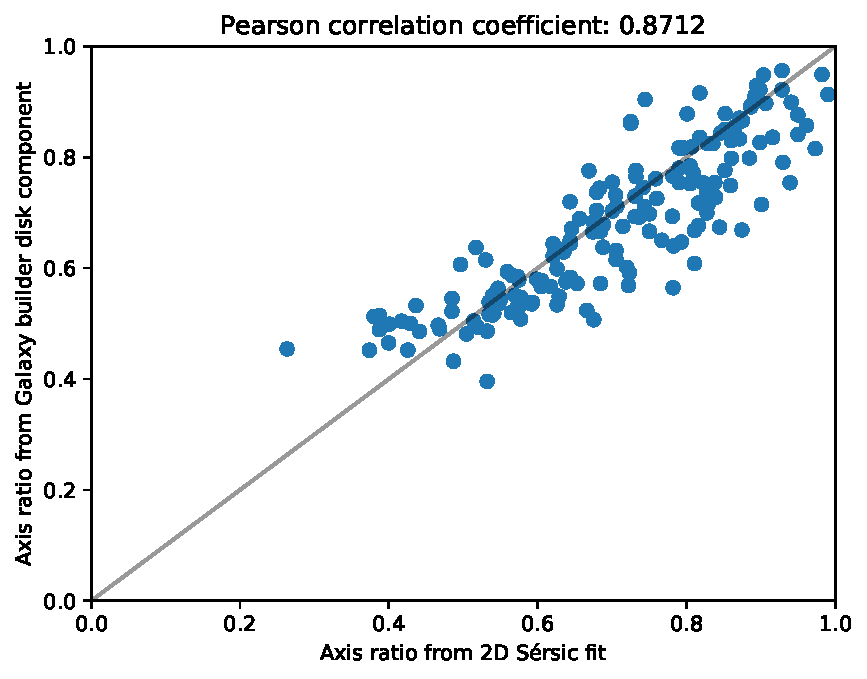
\includegraphics[width=8cm]{images__results/GZBvsNSA_ax-ratio_SERSIC_BA.pdf}
  \caption{Comparison between the axis ratios of the disk components of aggregated Galaxy Builder models to the results of an r-band S\'ersic profile fit.}
  \label{fig:ax_ratio_comparison}
\end{figure}

We also make comparisons to existing measures of morphology for individual galaxies. Using morphology results from GZ2, we can investigate how likely a volunteer is to incorporate a bulge or bar component in their model relative to its existing morphological classification obtained through citizen science.

Mirroring \citet{Kruk2017:1710.00093v2}, we define a galaxy as disk dominated if the debiased GZ2 fractions

\begin{equation}
p_\mathrm{no\; bulge} + p_\mathrm{just\; noticeable} > p_\mathrm{obvious\; bulge} + p_\mathrm{dominant\; bulge},
\end{equation}

or bulge dominated if the converse. Grouping our galaxies based on their type, we find that the probability of a classification of a disk dominated galaxy having a bulge was \comment{$0.7293 \pm 0.0781$}, whereas for a bulge dominated galaxy it was \comment{$0.7707 \pm 0.0806$}. Inspection of resulting aggregated models from Galaxy Builder suggests that many volunteers were using a highly elliptical bulge component to model light in both a galaxy's bulge and its bar, it is possible that enforcing a circular bulge may have provided more consistent classifications and less ambiguity for volunteers.

When comparing the probability of a classification containing a bar component against a galaxy being classed as strongly-barred or as having no bar (as defined in \citealt{Masters2010:1003.0449v2}), we see a significant difference: classifications of strongly-barred galaxies ($p_\text{bar} > 0.5$) had a \comment{$0.5713 \pm 0.1549 \%$} chance of containing a bar, vs \comment{$0.3666 \pm 0.1147\%$} for galaxies classed as having no bar ($p_\text{bar} < 0.2$). The Spearman correlation between GZ2's $p_\text{bar}$ and the bar likelihood in Galaxy Builder is \comment{$0.751$}. \comment{what does this statistic mean?}


\subsubsection{Aggregated Spiral Arms}
In order to benchmark the reliability of this method of spiral parameter extraction, we compare the result of our logarithmic spiral fit to the relationship obtained by \citet{Hart2016:1607.01019v1} between GZ2 classification and galaxy pitch angle (Figure \ref{fig:hart_pitch_angle}). Their fit was obtained using a leading automated spiral arm detection and fitting tool, \textsc{SpArcFiRe} \citep{Davis2014:1402.1910v1}. We find good agreement, although there are large error bars on the GZ2-produced pitch angle (and a the caveat in the paper that these pitch angles should not be used for individual galaxies).

\begin{figure}
  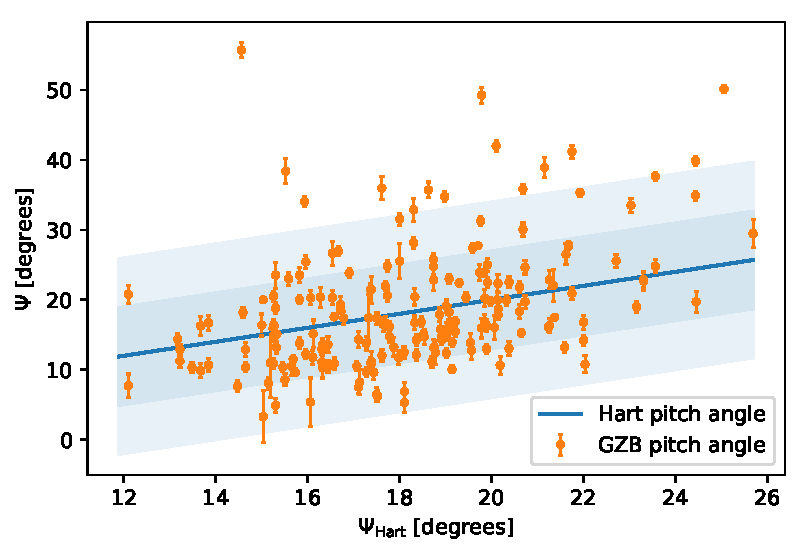
\includegraphics[width=8cm]{images__results/pitch-angle-comparison.pdf}
  \caption{A comparison of Pitch angle obtained by \citet{Hart2016:1607.01019v1} with measured pitch angles for the aggregated model results in galaxies in the Galaxy Zoo Builder sample. Errors on the Galaxy Builder pitch angles come from dispersion in the arms drawn by volunteers.}
  \label{fig:hart_pitch_angle}
\end{figure}

We can also directly compare the pitch angles from Galaxy Builder models to the output of the SpArcFiRe software, as shown in Figure \ref{fig:sparcfire_pitch_angle}. The SpArcFiRe pitch angle used is the length-weighted mean of all arms of the dominant chirality of a galaxy. In this plot, unlike Figure \ref{fig:hart_pitch_angle}, errors are the sample error of arms used in the averaging and is a measure of inter-arm variation pitch angle.
\begin{figure}
  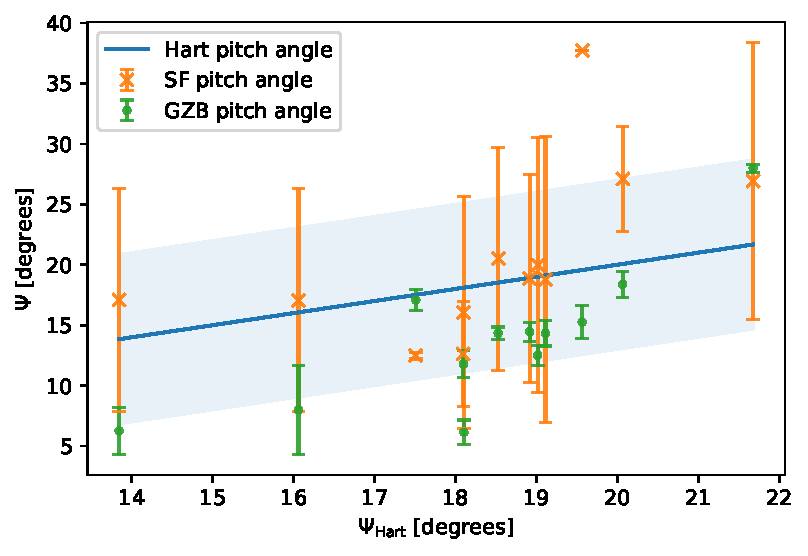
\includegraphics[width=8cm]{images__results/pitch-angle-comparison2.pdf}
  \caption{A comparison between pitch angles obtained by \citet{Hart2016:1607.01019v1} (blue line) to those obtained through Galaxy Builder and SpArcFiRe. Errors are the sample error of arms used in the averaging and is a measure of inter-arm variation pitch angle.}
  \label{fig:sparcfire_pitch_angle}
\end{figure}


\subsubsection{Comparison to Photometric Fits}
In this Section we make comparisons between Galaxy Builder models and the result of many-component photometric fits. \citet{Kruk2017:1710.00093v2} performed many-component, multi-band decompositions of a selection of Sloan galaxies, 12 of which were also classified in Galaxy Builder. For each of these galaxies we obtain the ``best'' model provided by volunteers (scored using mean squared error, in units of nanomaggies) and futher optimize the slider parameters available to volunteers, as well as the effective radius and axis ratio of all components. Figure \ref{fig:sd_comp_comparison}.

\begin{figure}
  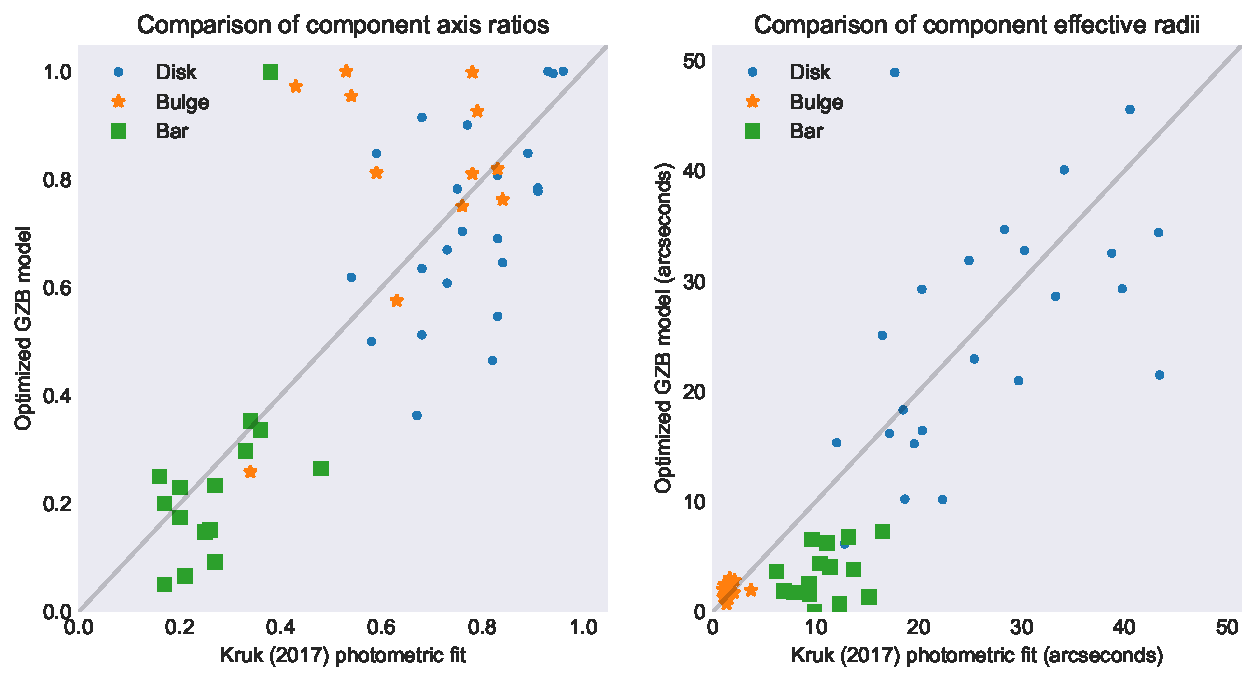
\includegraphics[width=8cm]{images__results/sd_comp_comparison.pdf}
  \caption{Comparison between optimized Galaxy Builder models and the result of 3\-component, multi\-wavelength fits performed by \citet{Kruk2017:1710.00093v2}.}
  \label{fig:sd_comp_comparison}
\end{figure}
\end{document}
